
\section{MSC}
\label{sc:MSC}
MSC ist eine vom ITU-T als Recommendation Z.120
standardisierte graphische Spezifikationssprache. Sie dient
zur Beschreibung des Kommunikationsverhaltens zwischen
Systemkomponenten und deren Umgebung. Die Kommunikation
wird durch den Austausch von Nachrichten (Messages)
spezifiziert.\cite{MT009} \\
Die MSC-Sprache hat sich aus den OSI Time Sequence
Diagrams zu einer vollst¨andigen graphischen Sprache
mit formaler Syntax und Semantik entwickelt.
Mit den Sequence Diagrams wurde eine Variante von MSC
in die UML integriert. Obwohl beide Sprachen auf den
gleichen Prinzipien beruhen, gibt es auf Grund der verschiedenen
Anwendungsbereiche unterschiedliche Sprachkonstrukte
und Unterschiede in der Darstellung. Durch eine
Kombination der St¨arken von MSC und den Sequence
Diagrams bem¨uht man sich zur Zeit verst¨arkt um eine Harmonisierung der beiden Diagrammarten.\\
In diesem Abschnitt werden die wichtigsten Konstrukte der
MSC-Sprache an Hand von MSCs1 für das in der Einleitung zu dieser Abschnittreihe beschriebene Beispiel erläutert. Das Beispiel beschreibt einen Produktionsprozess, in dem eine Produktionszelle aus vier verschiedenen Einzelteilen vom Typ A, B, C und D zwei Produkte vom Typ AC und BDC herstellt.


\subsection{Basic-MSC}
Basic-MSC umfasst alle Sprachkonstrukte, die notwendig sind, um den Nachrichtenfluss zu spezifizieren. Diese
Sprachkonstrukte sind: Instanz, Message, Environment, Action, Timer-Start, Timeout, Timer-Stop, Create, Stop und
Condition.\cite{MT009} \\

\begin{center}
\begin{figure}[h]
   

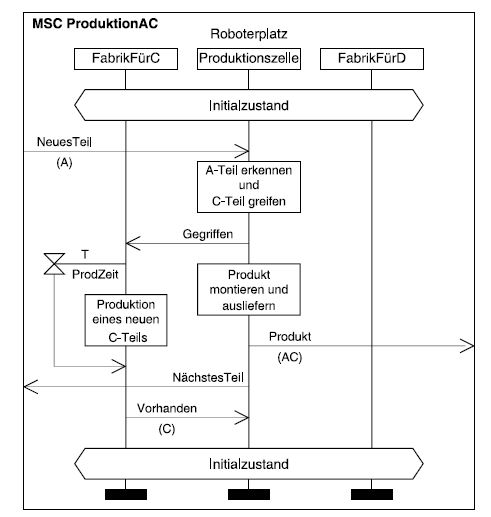
\includegraphics[scale=1]{Graphics/MSC1.jpg}

\captionof{figure}{Ein Basic-MSC }


Quelle : \cite{MT009}
Part 1: Message Sequence Chart (MSC) 

 
\label{fig7}


\end{figure}

\end{center}
\newpage
Ein Basic-MSC mit dem Namen ProduktionAC ist in
Abbildung 1.6 gezeigt. Es beschreibt die Produktion eines aus einem
A- und einem C-Teil zusammengesetzten Produkts.
Das MSC abstrahiert von den Details und zeigt nur den Informationsaustausch
zwischen den drei Hauptkomponenten
des Produktionsprozesses: Der Produktionszelle und den
zwei Fabriken für C- und D-Teile.
\\
Der Produktionsprozess befindet sich zu Beginn in seinem
Initialzustand: Das System ist initialisiert und Teile
der Typen C und D sind gefertigt, eingelagert und der
Produktionszelle zur Verfügung gestellt worden. Die Systemumgebung
übergibt ein A-Teil an die Produktionszelle.
Diese erkennt den Typ des Teils, greift das für die Produktion
notwendige C-Teil und meldet das Entfernen des
C-Teils vom Greifplatz an die Fabrik, die C-Teile herstellt.
Ein Produkt vom Typ AC wird gefertigt und dann
ausgegeben. Danach meldet die Produktionszelle die Bereitschaft
für die Bearbeitung des nächsten A- oder B-Teils
an die Systemumgebung. Parallel zu den Aktionen der Produktionszelle
wird ein neues C-Teil produziert und zur
Verfügung gestellt.\cite{MT009} \\
\subsubsection{Instanz und Message}
Die wichtigsten Sprachkonstrukte von Basic-MSC sind Instanz
und Message. Instanzen sind Komponenten, die untereinander
oder mit der Systemumgebung asynchron Messages
austauschen können.\\
In der graphischen Form werden Instanzen als vertikale
Linien oder alternativ als Säulen dargestellt. Innerhalb
des Instanzkopfes wird der Instanzname spezifiziert,
zus¨atzlich kann ein Typ angegeben werden (z.B. Instanz
Produktionszelle vom Typ Roboterplatz in
Bild 1). Das Ende einer Instanz kann durch ein Instanz-
Ende-Symbol beschrieben werden. Ein Instanz-Ende
bedeutet nicht, dass die Instanz gestoppt ist, sondern lediglich
dass in dem MSC keine weiteren Ereignisse für die
Instanz beschrieben werden.\\
Messages werden durch Pfeile dargestellt. Diese Pfeile
k¨onnen horizontal oder geneigt sein, um den Zeitverlauf
anzuzeigen. Eine Message definiert zwei Ereignisse: Der
Pfeilanfang beschreibt das Senden und die Pfeilspitze bezeichnet
die Verarbeitung einer Message. Die Beschriftung
einer Message besteht aus ihrem Namen und optionalen
Message-Parametern, die in Klammern angegeben werden
m¨ussen (z. B. Message NeuesTeil mit dem Parameter A
in Abbildung 1.6).\\
Entlang jeder Instanzachse wird eine Totalordnung der spezifizierten
Message-Sende- und Message-Verarbeitungsereignisse
angenommen. Ereignisse auf verschiedenen Instanzachsen
werden durch Message-Kommunikation partiell
geordnet, da eine Message zuerst gesendet werden muss,
bevor sie verarbeitet werden kann.\cite{MT009}
\subsubsection{Environment}
Die Diagrammfläche eines MSC wird durch einen rechteckigen
Rahmen begrenzt. Der Diagrammrahmen definiert
die Systemumgebung und heißt Environment. Messages,
die aus der Systemumgebung kommen oder an die Systemumgebung
gesendet werden, beginnen und enden auf
dem Environment (z.B. die Messages NeuesTeil und
Produkt in Bild 1). Im Gegensatz zur Totalordnung entlang
der Instanzachsen ist für Sende- und Verarbeitungsereignisse
auf dem Environment keine Ordnung definiert.\\
\subsubsection{Action}
Zusä¨atzlich zur Message-Kommunikation können Aktionen
von Instanzen in Form von Actions spezifiziert werden.
Eine Action wird durch ein Rechtecksymbol dargestellt, das
beliebigen Text enthalten kann (z. B. Action ,Produkt
montieren und ausliefern‘ in Abbildung 1.6).\\
\subsubsection{Timer}
Zur Beschreibung von Timern bietet MSC die Sprachkonstrukte
Timer-Start, Timeout und Timer-Stop an. Timer-Start
spezifiziert das Setzen, Timeout den Ablauf und Timer-Stop das Zur¨ucksetzen eines Timers. In MSC ist ein Timer
immer einer Instanz zugeordnet. Die graphischen Timer-Symbole sind daher immer mit der dem Timer zugeordneten
Instanz verbunden.\\

Ein Timer-Start wird durch ein mit der Instanzachse
verbundenes Sanduhr-Symbol dargestellt. Ein zugehöriges
Timeout wird durch einen Pfeil beschrieben, der am
Sanduhr-Symbol beginnt und auf der Instanzachse endet.
Ein Timer-Stop wird durch ein mit der Instanzachse verbundenes
Kreuz beschrieben. Ein Timersymbol wird mit
dem Timernamen und optional mit Timer-Parametern versehen.
Ein Timer-Start und das zugeh¨orige Timeout werden
in Bild Abbildung 1.6 verwendet, um die Produktionszeit für ein Teil des
Typs C zu modellieren. Der Timer hat den Namen T und
den Parameter Prodzeit, der die Laufzeit des Timers
spezifiziert.\\
\subsubsection{Condition}
Eine Condition beschreibt einen Zustand, der sich auf
eine Menge der im MSC enthaltenen Instanzen bezieht.
Graphisch werden Conditions durch Sechsecke dargestellt,
die die Instanzen, auf die sich die Condition bezieht,
¨uberdecken. Conditions werden zur Beschreibung von
wichtigen Systemzuständen benutzt. In Bild Abbildung 1.6 befinden sich
zwei Conditions, die beide den globalen Systemzustand
Initialzustand beschreiben.\\
\subsubsection{Create und Stop}
Die MSC-Sprache enthält die Konstrukte Create und Stop
für die dynamische Erzeugung und Terminierung von Instanzen.
Ein Create wird durch einen gestrichelten Pfeil
mit optionalen Parametern beschrieben. Ein Create-Pfeil
beginnt an der Erzeuger-Instanz und endet am Kopf der erzeugten
Instanz. Eine Instanz kann sich selbst durch eine
Stop-Aktion terminieren. Ein Stop wird graphisch durch ein
Kreuz am Ende der Instanzachse spezifiziert.\\

\subsection{Strukturelle Sprachkonstrukte}
Strukturelle MSC-Sprachkonstrukte bezeichnen Sprachelemente,
die über die Beschreibung des reinen Messageflusses
hinausgehen. Mit ihnen lassen sich MSCs und
MSC-Teile zu komplexeren Abläufen kombinieren (Inline-
Expressions und High-Level-MSC), MSC-Diagramme in
anderen MSC-Diagrammen wiederverwenden (References),
MSC-Instanzen verfeinern (Decomposition) und allgemeine
Ereignisstrukturen für Instanzen definieren (Coregion und
General Ordering). Aus Platzgründen kann im Rahmen
dieses Artikels nur auf Inline-Expressions, References und
High-Level-MSC (HMSC) eingegangen werden.\cite{MT009}\\

\begin{center}
\begin{figure}[h]
   

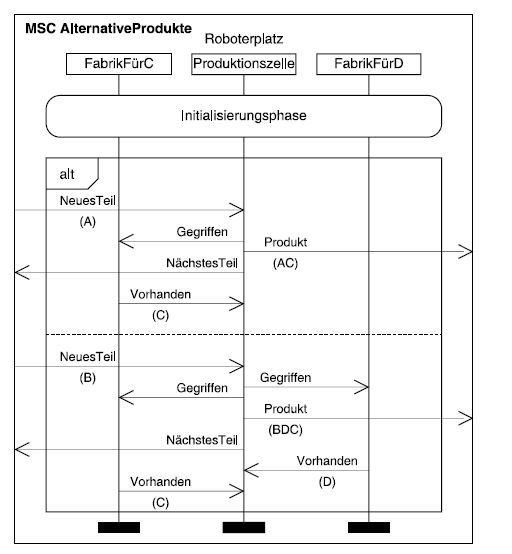
\includegraphics[scale=1]{Graphics/MSCmit.jpg}

\captionof{figure}{MSC mit strukturellen Sprachkonstrukten }


Quelle : \cite{MT009}
Part 1: Message Sequence Chart (MSC) 

 
\label{fig8}


\end{figure}

\end{center}
\newpage
\subsubsection{Inline-Expressions}
Mit Inline-Expressions können Teilabl¨aufe, die innerhalb
eines MSC-Diagramms spezifiziert worden sind, zu komplexeren
Abläufen kombiniert werden. Für die Kombination
bietet MSC die Operatoren alt, par, loop, opt und exc an. Sie erlauben es, die Wiederholung von Teilabläufen
(loop-Operator), alternative Teilabl¨aufe (alt-Operator), die
parallele Komposition von Teilabläufen (par-Operator), optionale
Teilabläufe (opt-Operator) und Ausnahmen in Form
von Teilabläufen (exc-Operator) zu spezifizieren. Graphisch
werden Inline-Expressions als Rechtecke mit gestrichelten
Linien als Separatoren f¨ur Teilabläufe dargestellt. Der Operator
wird in der linken oberen Ecke spezifiziert.
Eine Inline-Expression mit einem alt-Operator befindet
sich in Abbildung 1.7 . Die alternativen Teilabläufe beschreiben
die Fertigung von Produkten der Typen AC und BDC in
Abhängigkeit des von der Systemumgebung übergebenen
Basisteils (A oder B).\cite{MT009} \\
\subsubsection{References}
References ermöglichen es, MSCs in anderen MSCs wieder
zu verwenden. Eine Reference referenziert ein anderes
MSC über dessen Namen, d. h. eine Reference kann als
Platzhalter für das referenzierte MSC angesehen werden.
Graphisch werden References durch ein Rechteck mit abgerundeten
Ecken dargestellt. Eine Reference befindet sich
auch in Abbildung 1.7 . Sie referenziert ein MSC mit dem Namen
Initialisierungsphase, das die Initialisierung
des Produktionsprozesses beschreibt.\\
\subsection{High-Level-MSC}
High-Level-MSC (HMSC) erlaubt es, die Kombination von
MSCs in Form eines gerichteten Graphen zu beschreiben.
Die Knoten eines HMSC-Diagramms sind ein Anfangsknoten, Endknoten, Konnektoren, References und Conditions.
\\ In HMSC konzentriert man sich auf die Darstellung
der Kombination von MSC-Diagrammen und abstrahiert
von den Instanzen und dem Messagefluss. HMSCDiagramme
werden häufig auch Roadmaps genannt. Mit
ihnen lässt sich die sequentielle, parallele und alternative
Kombination von MSCs in einer sehr intuitiven Form beschreiben.\\

\begin{center}
\begin{figure}[h]
   

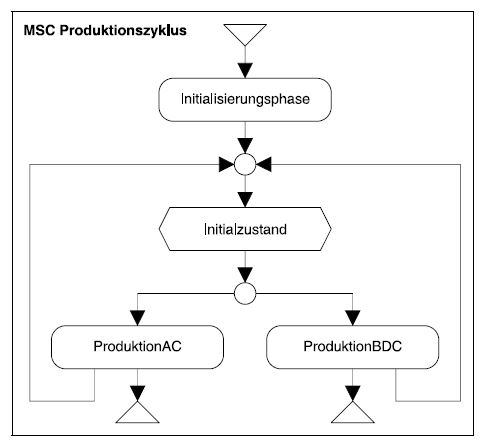
\includegraphics[scale=1]{Graphics/HMSC.jpg}

\captionof{figure}{Ein High-Level-MSC }


Quelle : \cite{MT009}
Part 1: Message Sequence Chart (MSC) 

 
\label{fig9}


\end{figure}

\end{center}
\newpage
Der HMSC in Abbildung 1.8 beschreibt die erwarteten AblÄufe
des Produktionsprozess-Beispiels: Nach der Initialisierungsphase
befindet sich der Produktionsprozess in seinem
Initialzustand. Im Initialzustand können entweder Produkte
vom Typ AC oder vom Typ BCD hergestellt werden. Nach
der Herstellung eines Produkts befindet sich der Produktionsprozess
wieder im Initialzustand und ein neues Produkt
kann gefertigt werden, oder der Produktionsprozess endet.

\subsection{Weitere Sprachkonstrukte}
In diesem Artikel konnten aus Platzgründen nur die
wichtigsten Elemente der MSC-Sprache vorgestellt werden.
Neben den genannten Konstrukten enthält MSC
noch einige weitergehende Konzepte, die MSC zu einer
vollständigen Spezifikationssprache machen: Die zu einer
Spezifikation gehörenden MSC-Diagramme können in
einem MSC-Dokument gesammelt und strukturiert werden.
MSC besitzt keine eigene Datensprache, aber eine
allgemeine Datenschnittstelle, die es erlaubt, Datenbeschreibungen
aus anderen Sprachen wie z. B. C, C++, SDL
oder Java zu benutzen. Zur Spezifikation von Realzeitanforderungen
können absolute Zeitpunkte und Zeitintervalle
in MSC-Diagrammen spezifiziert werden. Weiterhin wurden
UML-Konzepte zur objektorientierten Modellierung,
wie z. B. Control-Flow und Procedure-Calls, übernommen.\cite{MT009}





